\documentclass[letterpaper, 10 pt, conference]{ieeeconf}  % Comment this line out
                                                          % if you need a4paper
%\documentclass[a4paper, 10pt, conference]{ieeeconf}      % Use this line for a4
                                                          % paper

\IEEEoverridecommandlockouts                              % This command is only
                                                          % needed if you want to
                                                          % use the \thanks command
\overrideIEEEmargins
% See the \addtolength command later in the file to balance the column lengths
% on the last page of the document

\usepackage[pdftex]{graphicx}
% TODO remember we need to meet color compliance:
% http://its.papercept.net/conferences/support/general.php

% TODO better name!
\title{\LARGE \bf
Approximately Orchestrated Road Traffic Automata:\\
Large-scale Traffic Simulation for Autonomous Vehicles
}

\author{Dustin Carlino, Mike Depinet, Piyush Khandelwal, and Peter Stone\\
        Department of Computer Science\\
        The University of Texas at Austin\\
        Austin, TX 78712\\
        {\tt \small\{dcarlino,msd775,piyushk,pstone\}@cs.utexas.edu}}

\long\def\commentp#1{{\bf **Peter: #1**}}
\long\def\commentpk#1{{\bf **Piyush: #1**}}
\long\def\commentm#1{{\bf **Mike: #1**}}
\long\def\commentd#1{{\bf **Dustin: #1**}}
\long\def\commentc#1{{\bf **Chiu: #1**}}

% \long\def\commentp#1{}
% \long\def\commentpk#1{}
% \long\def\commentm#1{}
% \long\def\commentd#1{}
% \long\def\commentc#1{}

\begin{document}

\maketitle
\thispagestyle{empty}
\pagestyle{empty}

%%%%%%%%%%%%%%%%%%%%%%%%%%%%%%%%%%%%%%%%%%%%%%%%%%%%%%%%%%%%%%%%%%%%%%%%%%%%%%%%

\begin{abstract} 

Autonomous vehicles have seen great advancements in recent years, and such
vehicles are now ever closer to being commercially available.  The advent of
driverless cars provides opportunities for optimizing traffic in ways not
possible before. This paper introduces an open source multiagent microscopic
traffic simulator called AORTA, which stands for \textit{Approximately
Orchestrated Road Traffic Automata}, designed for optimizing autonomous traffic
at a city-wide scale. AORTA creates scale simulations of the real world by
generating maps using publicly available road data from \textit{OpenStreetMap}
(OSM). This allows simulations to be set up through AORTA for a desired region
anywhere in the world in a matter of minutes. AORTA allows for optimizing
traffic by creating more intelligent behaviors for individual drivers (agents),
as well as by defining new intersection policies that can be followed by these
autonomous agents. These agent behaviors define how agents interact with one
another, follow intersection policies, and select the next action to take. This
paper demonstrates a simple applications using AORTA through an experiment
testing an intersection policy designed for autonomous vehicles at a city-wide
scale.

\end{abstract}

%%%%%%%%%%%%%%%%%%%%%%%%%%%%%%%%%%%%%%%%%%%%%%%%%%%%%%%%%%%%%%%%%%%%%%%%%%%%%%%%

\section{INTRODUCTION}
\label{sec:introduction}

% theme: easy simulation in your city, in 2 minutes!
% be sure to emphasize open source!
% contribution: autonomous car / human car sim on EXISTING INFRASTRUCTURE

Autonomous vehicle technology has made tremendous progress in the last decade.
In 2004, the farthest distance traveled by a vehicle autonomously in the DARPA
Grand Challenge was 11.9km \cite{cnnGrandChallenge2004}. By 2007, six of the
competing teams completed the 96km course set for the DARPA Urban Challenge
\cite{spectrumUrbanChallenge2007}. They did so while following the same traffic
laws followed by human drivers, navigating along with other moving vehicles,
and following correct intersection precedence order. Since then, Google's
driverless cars have clocked more than 250,000km on public roads in urban
California, USA \cite{tedThrun2011}. In 2010, researchers from the University
of Parma successfully completed an autonomous \textit{intercontinental} run
from Parma, Italy to Shanghai, China \cite{cnnVislab2010}. The successful
completion of all these milestones suggests that autonomous cars are here to
stay, and are ever closer to becoming commercially available. With the arrival
of autonomous cars, it also becomes possible to optimize traffic in ways not
possible for human drivers. 
\commentd{If we need space, I agree with Dr Chiu, some of this could be trimmed}

% The arrival of driverless cars presents several challenges that need to be
% addressed in the near term. Road infrastructure changes could provide important
% improvements to traffic involving autonomous vehicles. A number of legal and
% safety concerns need to be addressed in the context of driverless cars. Human
% drivers need new methodologies to interact with autonomous drivers on public roads.
% This work aims to solve some of these problems by providing a sandbox in which such
% methodologies can be found and tested for safety and efficiency before being
% deployed in the real world.  In this manner, the present work aids in the effort to find
% intermediate stages between entirely human and entirely autonomous traffic.

\begin{figure}[t]
  \centering 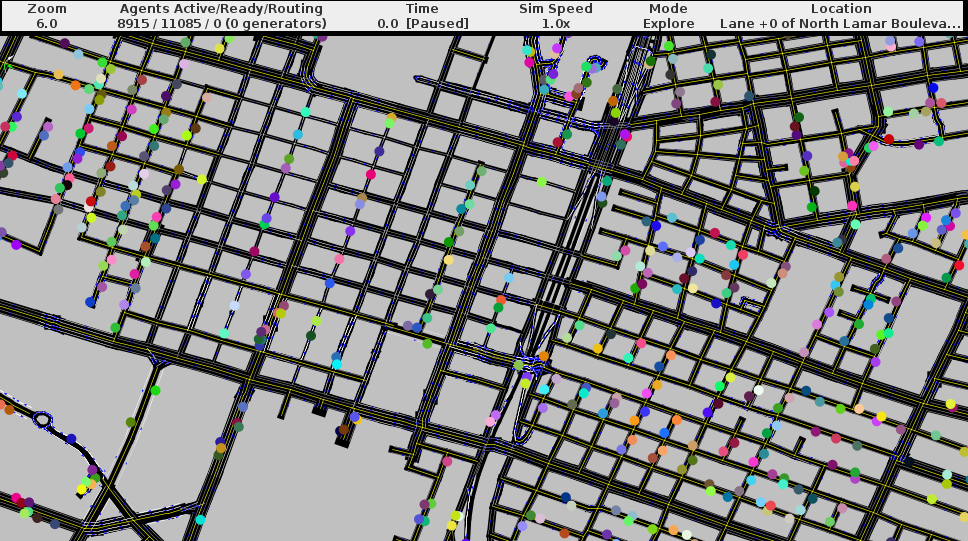
\includegraphics[width=\linewidth]{downtown_atx.png}
  \caption{A simulation of downtown Austin, Texas.}
  \label{fig:ui_screenshot}
  \vspace{-15pt}
\end{figure}

% TODO reference the screenshot

This paper introduces an open source multigent microscopic traffic simulator
called AORTA, which stands for \textit{Approximately Orchestrated Road Traffic
Automata}, a platform designed for testing autonomous vehicle behaviors and
intersection policies. Autonomous vehicles, termed agents, use
behaviors to interact with one another, follow intersection policies, and
decide on both long term and short term actions. AORTA allows for the creation
of intersection policies that designate when agents can cross the
intersection. AORTA's goal is to allow for the definition of new agent
behaviors and intersection policies to optimize autonomous traffic.
Additionally, by assigning human-like behaviors such as the ``car following
model'' \cite{brackstone1999car} to agents, and traffic-signal-like policies to
intersections, AORTA could potentially simulate human traffic.
\commentd{Previously, ``AORTA allows for the creation
of intersection policies on top of a reservation based intersection manager
\cite{JAIR08-dresner}, and these policies designate when agents can cross the
intersection.'' Actually, reservations are just one policy. Do we want to focus
on the general case here, or autonomous specifically?}

Like any other microscopic traffic simulator, AORTA needs maps to run
simulations. One of AORTA's key features is that it generates maps using real
road data available from OpenStreetMap (OSM) \cite{osm}, a moderated,
user-editable interface for world maps. A map for any desired city in the world
can be downloaded, which is then parsed by AORTA to set up a scale simulation of
the real world in a few minutes. AORTA is available open-source and is easily
extensible \footnote{Code available at
\texttt{http://code.google.com/p/road-rage}} \commentpk{could also change this
to a citation}, making it easier for users to test out a number of agent
behaviors and intersection policies.

This paper explores the state-of-the-art in traffic simulators in section
\ref{sec:related_work}, followed by a description of AORTA's architecture in
section \ref{sec:arch}.  Use of OSM data in AORTA is explained in section
\ref{sec:map}, along with a description of the simulator and the default
behaviors available in AORTA in section \ref{sec:simulation}. An experiment
investigating the benefit of an alternate intersection policy designed for
autonomous vehicles is presented in \ref{sec:results}. The paper then concludes
with a discussion on future work.

%%%%%%%%%%%%%%%%%%%%%%%%%%%%%%%%%%%%%%%%%%%%%%%%%%%%%%%%%%%%%%%%%%%%%%%%%%%%%%%%

\section{RELATED WORK}
\label{sec:related_work}

% just draw differences between us and them

Computational processing power has made excellent advancements in the last two
decades. Parallel computing and the use of GPUs have enabled microscopic models
of traffic simulation to generate results at a meaningful scale (city-wide or
greater) \cite{nagel1994microscopic,shen2011agent}. As a result, a number of
multiagent micro-simulators have been introduced in the past decade. We review
relevant simulators and other related work in this section.

OSM data has been used by traffic simulators in the past. MATSim is one such
multiagent simulator that focuses on performing large-scale simulations in a
relatively small amount of time \cite{balmer2009matsim}. Traffic demand is
supplied to MATSim in the form of \textit{plans} that an individual may intend
to follow in a given day. MATSim aims to iteratively improve these plans though
offline computation to maximize traffic throughput. In other words, it helps
individuals understand the best way to go about their daily routine to minimize
time spent in transit. This goal is somewhat different from that of AORTA,
where the demand supplied by individuals is taken as is. Rather than simply
improving routes, AORTA allows creating entirely different behaviors for both
vehicles and intersections.

Another popular open source traffic simulator that can use OSM data is SUMO
\cite{SUMO2011}, which shares the similar goals as AORTA. SUMO has been used to
study the effect of automated transportation systems, route planning of
individual vehicles, as well as dynamically adapting traffic signal policies to
increase traffic efficiency.  AORTA and SUMO differ in the manner in which
intersections are handled. SUMO uses traditional traffic signals, while AORTA
adopts a much more general \textit{reservation} system. A reservation tells a
car when it is safe to take its desired path through the intersection.
Reservations can be allotted to vehicles through more traditional means such as
traffic signals or stop-sign based intersection precedence, or through more
efficient methods designed specifically for autonomous vehicles
\cite{JAIR08-dresner}.
\commentd{Again, ``reservation'' feels like an overloaded term here, meaning the
general notion of being able to cross, as opposed to the specific policy.}

Efforts have been made to optimize traffic flow in the context of autonomous
vehicles. AIM \cite{JAIR08-dresner} is one such approach that aims to optimize
traffic flow of autonomous vehicles at a given intersection. The AIM approach
has been applied to a regular grid of four intersections
\cite{IROS11-hausknecht}, while AORTA has the potential to apply some of the
same research at a city-wide scale to real-world road networks.

Simulators have also focused on autonomous vehicles with sensors and actuators
\cite{figueiredo2009approach}. These simulators are used to ensure that
autonomous vehicles are behaving correctly while interacting with other
vehicles and infrastructure, given their configuration of sensors and
actuators. On the other hand, AORTA assumes that autonomous vehicles have
reasonable sensory input and mechanical output, and instead focuses on
interactions between an agent and its surrounding agents and intersections.

Autonomous agents have also been used in the past to model human traffic. For
instance, one approach models human merging and lane changing behavior through
the use of autonomous agents interacting with one another
\cite{hidas2002modelling}. Another approach attempted to improve traffic
congestion for human drivers by using a network of autonomous intersections.
These intersections have the ability to interact with one another and execute a
dynamic traffic signal policy minimizing overall wait time
\cite{manikonda2001autonomous}.

%%%%%%%%%%%%%%%%%%%%%%%%%%%%%%%%%%%%%%%%%%%%%%%%%%%%%%%%%%%%%%%%%%%%%%%%%%%%%%%%

\section{ARCHITECTURE}
\label{sec:arch}

% Diagram made with gliffy.com. architecture.gxml should enable editing.
\begin{figure}
  \centering 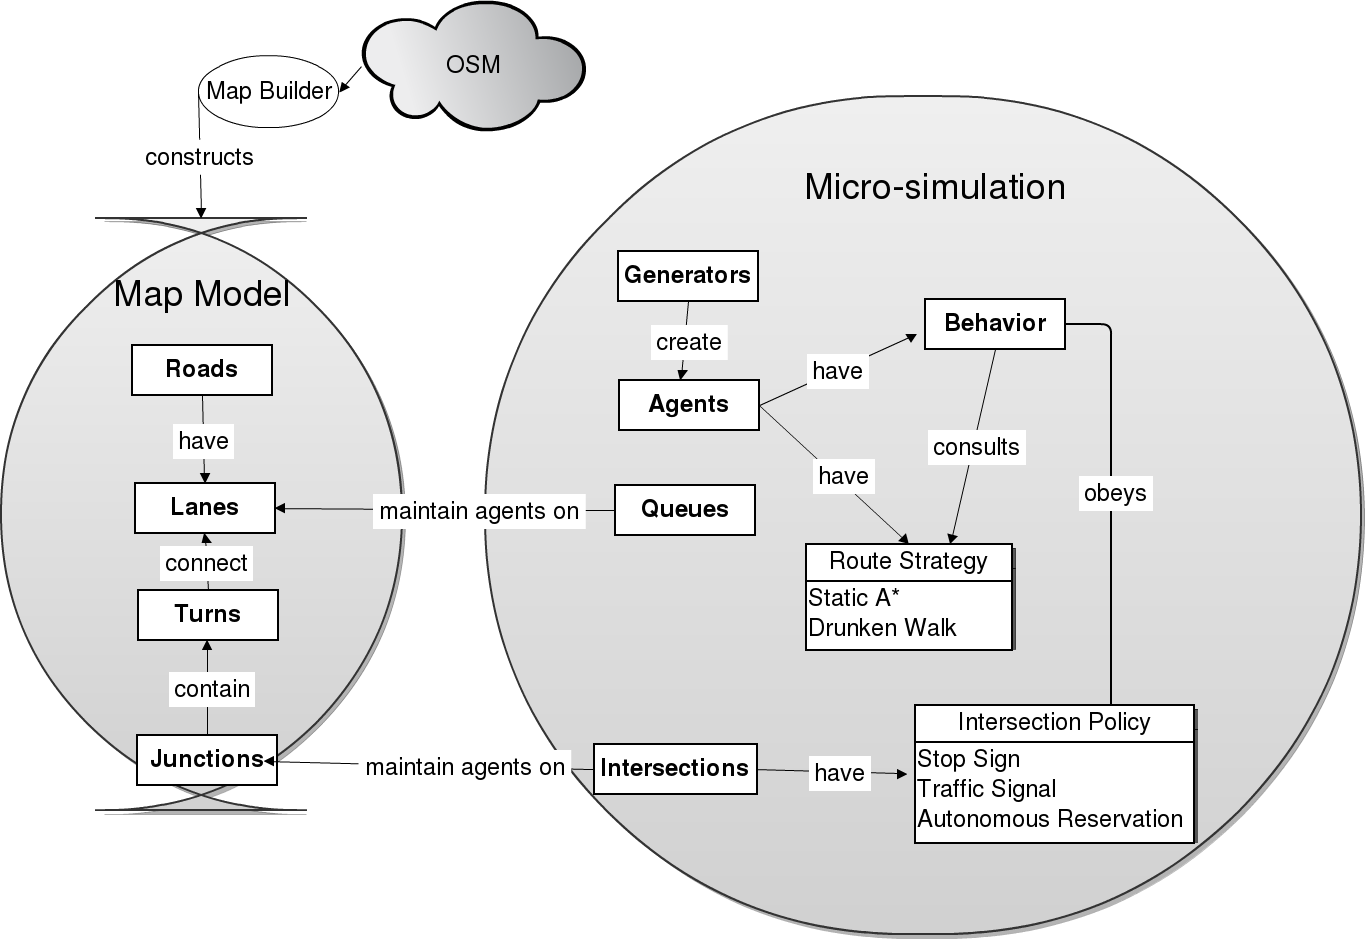
\includegraphics[scale=0.3]{architecture.png}
  \caption{A summary of AORTA's components.}
  \label{fig:arch}
  \vspace{-20pt}
\end{figure}

AORTA is divided into three modular components: the map model, micro-simulation
engine, and user interface (UI). The map model transforms OSM maps into AORTA
graphs, then answers pathfinding and geometry queries. The simulation engine
adds a notion of agents, vehicle dynamics, and collisions. Finally, the UI can
interactively render the map and agents. A headless mode also enables running
experiments without the overhead of visualization. The interaction between
modules is visualized in figure \ref{fig:arch}.

AORTA's implementation uses Scala, a language implemented on the Java Virtual
Machine \cite{scala}. Scala provides the advantage of functional programming
constructs while still permitting imperative style.  Extensions and clients
built on top of AORTA can be written in either Java or Scala. The software is
open-source and easily extensible. For instance, the stop sign sign policy used
in experiments described in section \ref{sec:results} is implemented in just 70
lines of code. 

Sections \ref{sec:map} and \ref{sec:simulation} describe map construction from
OSM data and the simulation engine used in the AORTA framework respectively.

%%%%%%%%%%%%%%%%%%%%%%%%%%%%%%%%%%%%%%%%%%%%%%%%%%%%%%%%%%%%%%%%%%%%%%%%%%%%%%%%

\section{MAP CONSTRUCTION FROM OSM}
\label{sec:map}

One of the key features of AORTA is the simulation of traffic on existing road
network data from OpenStreetMap \cite{osm}. The data from OSM is not directly
suitable for running a simulation and is pre-processed through a \emph{map
builder} utility. The map model generated by the builder is described in sec.
\ref{sec:mapmodel} and the process of refining OSM data is enumerated in sec.
\ref{sec:mapconstruction}.

\subsection{Map Model}
\label{sec:mapmodel}

\commentpk{I remember you guys mentioning there was a paper for SUMO describing
a similar process, we should ref it as to why OSM data is not directly suitable}
\commentd{We cite it in the conclusion because they had similar critiques about
  OSM. I don't think we have a source for why OSM isn't directly suitable,
  although that source also describes a conversion process.}

% \pix{map_model.png}
%    {Roads contain several lanes, and intersections contain several turns
%     between lanes.}
%    {scale=0.5}

A map is represented as a directed graph with \emph{lanes} as edges and
\emph{turns} as vertices. A \emph{road} groups a set of lanes together, one set
for each direction of travel. \emph{Intersections} map the possible turns from
incoming to outgoing lanes.  Since both lanes and turns support traffic, they
are grouped together as \emph{traversables}, meaning agents may exist on them.
\commentc{What about parking lots?}
\commentd{They're not something relevant for us to model. I don't think we need
to mention this.}

The map also has a geometric interpretation, used for visualization and
measuring physical distances. A road contains a sequence of points, defining
the center line that divides the road into two directions of travel. AORTA
interprets these points as straight lines and projects parallel lanes out using
a fixed width. Turns are modeled with a single straight line connecting the end
of one lane to the start of another. \commentc{Illustrate through a figure?}
\commentd{maybe a subfloat by the turn conflicts, sure}

\subsection{Map Construction Passes}
\label{sec:mapconstruction}

The builder works incrementally while parsing OSM graphs into the map model,
with each pass feeding the next. The map model is then stored in an XML format.
\begin{enumerate}
  \item OSM encodes many paths besides driveable roads, so the builder first filters
        these out. Next, the builder marks OSM nodes common to multiple roads, since
        they implicitly indicate intersections. Overpasses do not share nodes
        with the roads they cross \cite{osmOverpass}.
  \item OSM \emph{ways} (sequences of nodes) include many
        intersections, so the builder next splits ways into undirected
        segments of roads between exactly two intersections.
  \item The builder multiplies undirected roads into directed lanes in each
        direction (unless the road is marked one-way). The builder guesses the
        number of lanes based on OSM's ``road type'' tag or an explicit number of
        lanes, when that data is available.
  \item The builder constructs turns between incoming and outgoing lanes at each
        intersection. The angle between the two lanes determines whether the turn is
        a left, right, straight, or U-turn. When several lanes all cross into fewer
        lanes, the builder forces merging of the rightmost lanes. 
  \item Because turns are heuristically placed, the graph is often disconnected.
        In order to ensure that an agent will be able to reach any point in the map,
        the builder removes all but the largest strongly connected component of the
        digraph. Disconnected lanes are spliced out of larger roads, leaving
        unappealing geometric gaps, but correctly ensuring connectivity for
        corner-case free pathfinding.
\end{enumerate}

%%%%%%%%%%%%%%%%%%%%%%%%%%%%%%%%%%%%%%%%%%%%%%%%%%%%%%%%%%%%%%%%%%%%%%%%%%%%%%%%

\section{SIMULATION}
\label{sec:simulation}

\commentd{Is this incomplete?}
Different elements of the simulator are described as follows:

\subsection{Simulation Dynamics} 

AORTA uses microscopic simulation, modeling individual drivers as point agents
with a simple acceleration-based dynamics model. Time is modeled discretely,
and an agent accelerates at a fixed rate for the duration of a ``step'' to
achieve a new position and velocity. Space is continuous, meaning agents occupy
a moving interval of a lane, rather than one fixed tile of the road. Each time
step lasts for the same fixed duration, and the simulation does the following
for each time step:

% \textit{dt}.
% This lets agents reason about how far they will travel for a given choice of
% acceleration before being able to choose a different acceleration. Setting
% \textit{dt} to the ``reaction time'' of a human driver may be appropriate for
% experiments modeling humans.
% 
% Each step, the simulation does the following:

\begin{enumerate}
  \item Introduces new agents into the map
  \item Updates the position and velocity of agents based on their choice of
        acceleration in the previous step
  \item Checks for collisions
  \item Allows each agent's behavior to choose an action for the next step
\end{enumerate}

\commentpk{need to check the ordering of above enumeration}

\subsection{Spawning new agents}

To introduce new agents into the simulation in real-time, users can create
\emph{generators} programatically or using the UI. The generator produces the
desired amount of traffic by initializing agents from random locations inside a
\textit{start} polygon to random destinations within a \textit{goal} polygon.
Users can draw these polyons by mouse in the UI, allowing specific traffic
patterns like rush-hour scenarios to be easily simulated. A generator polygon
may also cover the entire map, uniformly distributing traffic everywhere.

Every step, a generator creates some number of new agents. If the agent's route
policy needs computation like pathfinding to operate, the generator either
performs it immediately (incurring a delay in simulation if it is running) or,
if possible, sends it to a pool of worker threads to process in the background.
Once an agent's route is ready, the agent waits alongside its starting lane (as
if it is in a driveway or parking lot). When the lane has no agents that could
potentially crash with the new vehicle, the new agent enters the system. % with
%zero initial speed. Because behaviors must enforce speed limit along a lane
%from the moment an agent enters a road, it is safe for a new agent to enter a
%road if there is no other agent within the worst-case distance (traveling
%distance at the speed limit, plus stopping distance from this speed) preceeding
%the spawn point. To avoid predicting which agents might enter the lane in the
%near future, there is a buffer space at the beginning of the lane where a new
%agent may never spawn. This disqualifies some short lanes from being spawn
%points, but this is not a big limitation in practice. \commentpk{I understand
%your concern about explaining the entire methodology, but the last 2 lines are
%unnecessary and somewhat distracting}

\subsection{Collision checking}

All traversables (lanes and the straight line-approximation of turns) maintain
an ordered queue of occupying agents. A collision is detected when two agents
reverse order after a time step has completed.

Intersections check for collisions by examining the turn each agent is
performing and verifying that no other agent is simultaneously performing a
conflicting turn. AORTA has a low-granularity model of turn conflict. If two
vehicles at any point along two different turns could ever come into contact,
then the turns are always in conflict, no matter where the agents actually are
along that turn. This is visualized in figure \ref{fig:conflicts}. Further work
is required before higher granularity can be introduced through space-time
tiling intersections \cite{JAIR08-dresner}, due to some of the complex
intersection geometries inferred from OSM \commentpk{If there is an image for
one such complex intersection geometry, we can place it next to the current fig
3 using a subfloat}.

% When a collision occurs, the simulator throws warnings and halts, since this
% indicates a bug in some policy. A future alternative could be to mark the region
% as impassable and re-route other traffic away from the accident.

\begin{figure}[h]
  \centering 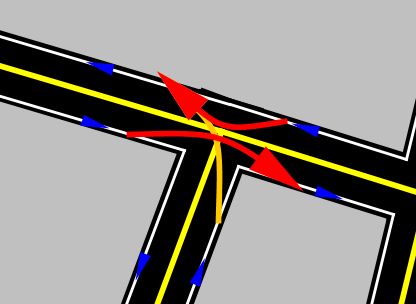
\includegraphics[scale=0.5]{turn_conflicts.png}
  \caption{An agent cannot turn left while agents on the perpendicular road cross}
  \label{fig:conflicts}
  \vspace{-15pt}
\end{figure}

\subsection{Agent Behaviors}

\commentd{Mike, I left off here.}

Each agent has a \emph{behavior} governing it, responsible for obeying
intersection policies and avoiding collisions. When the agent travels past the
end of a lane during its step, the behavior picks the turn to take. At each
step, the behavior can make the agent react by performing one of two actions:
disappearing from the map (when the agent is at rest and is done with its route)
or setting an acceleration for the next step.

\subsection{Intersection Policies}

A behavior's interaction with an intersection policy amounts to polling it with
the turn the agent wants to perform, the distance away the agent currently is,
and how long the agent has been waiting (so policies can enforce a required
delay before entering the intersection). The intersection policy simply orders
the agent to ``stop'' or ``proceed.'' \commentd{I'm not sure this fits in the
default behavior later anymore; just delete it?} The acceleration chosen to
avoid entering an intersection attempts to account for crosswalks by ending a
configurable threshold before the end of a traversable.

\subsection{Simulation Limitations}

Currently agents cannot change lanes. However, AORTA supports roads forcibly
merging by treating the merge point as an intersection. The lack of
lane-changing causes a second issue: gridlock.

Agents maintain a safe following distance from the next agent. If a lane is
filled, then an agent may be forced to stop in an intersection mid-turn and
block other traffic. The default behavior prevents this by refusing to start a
turn before the lookahead engine guarantees no agent will trigger a premature
stop.

However, with very high volumes of traffic, it is possible for waiting agents to
accumulate and fill lanes to their capacity. When this happens in a circular
manner so that the agent at the front of each lane is waiting to perform a turn
into another full lane with the same such head agent, gridlock \cite{AAAI11-au}
occurs; no agent in the system will make progress unless an agent at the front
decides to pick a different turn. Figure \ref{fig:gridlock} demonstrates this.
AORTA can detect this by finding cycles in the graph of the ``is following''
relation.

\begin{figure}[h]
  \centering 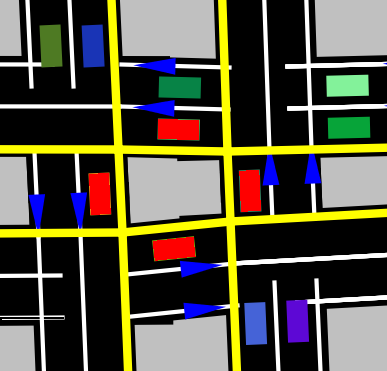
\includegraphics[scale=0.25]{gridlock.png}
  \caption{Each of the red agents wants to turn left, so none of them
           can. The traffic jam will slowly build up around this intersection.}
  \label{fig:gridlock}
  \vspace{-10pt}
\end{figure}

In many observed cases, the gridlock is caused by AORTA's present lack of
lane-changing support: agents loop around these intersections in order to enter
a lane adjacent to their original lane. Since these routes are still legal, it
is desirable to prevent or mend this without forcing different routes. However,
choosing alternative moves (by changing lanes or rerouting) is one sufficient,
but not necessarily required, condition for liveness \cite{AAAI11-au}.
\commentd{I misinterpreted the results of the paper originally. Is this a safer
and more relevant claim to make?}

\subsection{Extending AORTA}
\label{sec:config}

There are three main configurable components of the simulation, each with at
least one existing implementation: agent behaviors, routing strategies, and
intersection policies.

Currently, all agents use a primary behavior that is a generalized, baseline
behavior that guarantees not to collide with another agent or enter an
intersection at the wrong time. Since it picks the highest safe choice of
acceleration at each step, it could easily be extended to mimic human drivers by
traveling at some random lesser acceleration or to optimize fuel efficiency
by tuning movement.

Intersection policies are one of the most interesting aspects of the simulation
to tweak, especially in light of autonomous vehicles. Current policies include
traditional stop signs, traffic signals, and an AIM-inspired autonomous
reservation system \cite{JAIR08-dresner}. The traffic signals are further
extensible by assigning groups of non-conflicting turns at each intersection
with some duration and offset. Future policies could include signals that adapt
timings and refinements to the autonomous reservation policy.
\commentc{You can mention about using optimized traffic signal timings generated
  by commercial traffic signal optimization packages such as SYNCHRO (cite
  Husch, D. and Albeck, J. (2004) Trafficware Synchro 6 User Guide, TrafficWare,
  Albany, California.)
}

To pick turns, agent behaviors consult a route strategy. Two simple
implementations exist already: a static route using A* \cite{astar} and a
drunken walk that probabilistically moves towards the destination.  Researchers
can experiment with dynamic replanning or hierarchial planning without modifying
any code other than creating a new route implementation. Route policies could
also interact with a single central manager to gain some sort of global insight or
with autonomous intersections to avoid congestion.
\commentd{I can cite a paper for hierarchial planning. As for why, the 2
  mentioned are just examples of future work we intend to do, and I want to make
  the point that implementing both would be easy from a software engineering
  perspective.}

%%%%%%%%%%%%%%%%%%%%%%%%%%%%%%%%%%%%%%%%%%%%%%%%%%%%%%%%%%%%%%%%%%%%%%%%%%%%%%%%

\section{EXPERIMENTAL RESULTS}
\label{sec:results}

A particular focus of AORTA is intersection policies. To demonstrate how much
policy affects the throughput of intersections and total performance of the
transportation system, three policies are evaluated: stop sign, traffic signal,
and autonomous reservation. Every intersection uses the same policy.

\subsection{Experimental Setup}

The experiment simulates a 6 by 7 mile slice of downtown Austin,
Texas\footnote{bounded by the Mopac and Springdale Road horizontally, and Oltorf
Street and Koenig Lane vertically}, for one hour. The step duration is fixed at
0.1 seconds. While the intersection policies vary, the agents spawned and their
routes remain the same. A generator creates one new agent every 1 simulation
second, with a uniformly random starting position and goal.
\commentd{Chiu asked about the distribution of incoming agents. Is ``uniformly
random start and end'' not clear?}

These experiments are deterministically reproducible. A seed for the
pseudo-random number generator, the input graph, and the generators'
configuration fully determine the outcome of any simulation \footnote{This
  determinism may break down when generators use worker threads, since routes
  may be computed in different orders, causing agents to enter the road at
different times.}. After setting up a scenario in the UI, users can save this
configuration for resimulation.

The speed of simulation depends on the step duration dt, the map size, and the
number of agents. A measure independent of these factors is the number of agent
steps per second. On a 2.4 GHz machine, this can be observed to average at about
150,000, a number comparable to existing simulators \cite{SUMOthesis}. When dt
= 0.1 seconds, this means 15,000 agents can be comfortably simulated in
real-time. Further optimizations are planned.

\subsection{Intersection Policies Evaluated}

Stop signs accept agents first-come, first-served, refusing agents until they
have idled at 0 speed for 1 second. This delay approximates human reaction time.

The traffic signal policy requires timings and groups of simultaneous turns for
each intersection. The heuristic evaluated uses standard turn groups (turns from
parallel incoming directions are scheduled simultaneously, and left turns are
grouped) and employs breadth-first search to propagate timings. The goal is to
synchronize green signals so agents in some lanes do not stop for several
intersections.
\commentd{chiu recommends more details with how we propagate timings. Thoughts,
Mike?}

\commentd{advice on wording?}
Finally, in anticipation of the advent of autonomous vehicles, an autonomous
reservation policy inspired by AIM \cite{JAIR08-dresner} is tested. This policy
groups agents with compatible turns together, allowing new agents to join
existing groups. To prevent one heavy direction of traffic from hogging the
intersection indefinitely, a timeout preemptively cycles through reservations.

\subsection{Results}

\begin{figure}[h]
  \centering 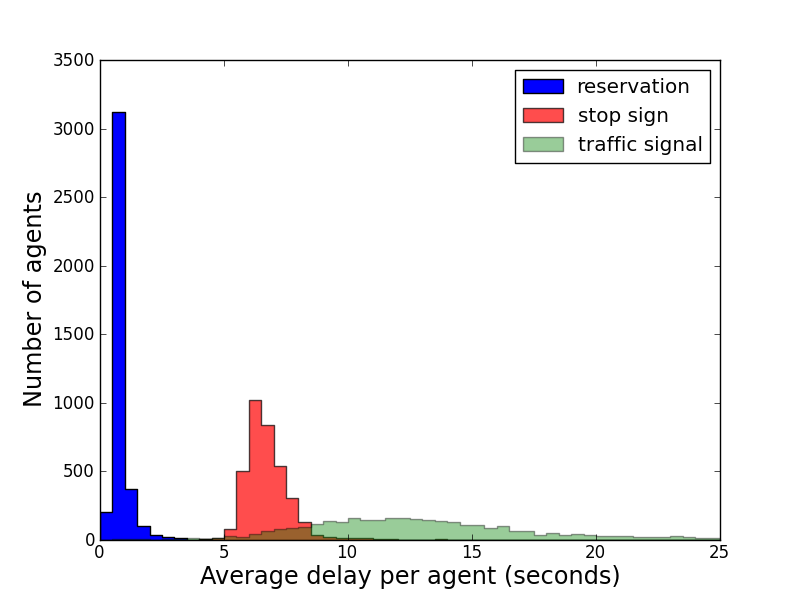
\includegraphics[width=\linewidth]{avg_lag_agent_atx.png}
  \caption{The distribution of average delay reveals that traffic signals can
           cause the most lag.}
  \label{fig:avg_lag}
  \vspace{-10pt}
\end{figure}
\commentc{This figure only shows the distributions for a particular
  traffic level only. People would wonder what is the traffic level.
Actually people are more interested to see how it varies with
different traffic levels so a few more graphs like this at
different traffic level is helpful.}
\commentc{Remove ``In this range'' in the y-label.}
\commentc{Replace ``lag'' with ``delay'' in the x-label}}

If an intersection immediately permits an agent to proceed and grants other
agents in the same lane similar access (because this new agent must still follow
these others), then the new agent may simply proceed at full speed limit without
pausing. This gives the least possible delay spent along some lane, so any extra
time is defined as lag and is used to measure intersection performance. Figure
\ref{fig:avg_lag} graphs the average of this delay per agent. On average,
reservation policies cause less than 1 second of delay at each intersection,
stop signs cause about 7 seconds lag, and traffic signals cause 16 seconds.
\commentd{We need to be clear that our traffic lights suck, so this number is
pretty biased.}

\commentc{Reviewers will certainly complain the lack of the details of the
  parameters you used, which implies your results can be somewhat ``biased''.
  Honestly, I don't think you should show this results in
  this paper because it is somewhere irrelevant to the topic.  Perhaps
  you should emphasize that these experiments intend to show what you can do
with your simulator.
}

\begin{figure}[h]
  \centering 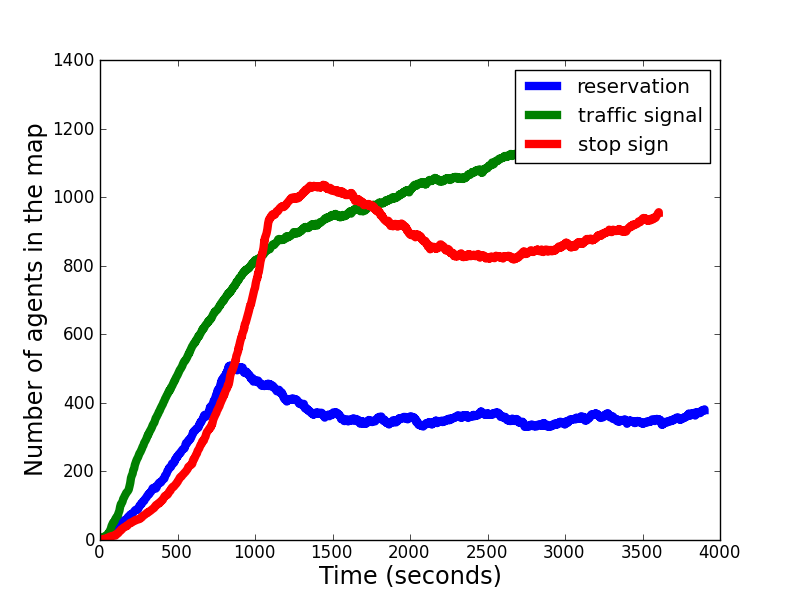
\includegraphics[width=\linewidth]{agent_cnt_atx.png}
  \caption{Autonomous reservations outperform stop signs, and traffic signal
           gridlocked. \commentc{This label is not helpful. Clarify ``active'' in y label.}}
  \label{fig:agent_cnt}
  \vspace{-10pt}
\end{figure}

The number of agents driving at some time changes because the continuous
generator introduces a new agent every second. This count reaches a steady
state when the generator introduces an agent at the same rate as older agents
finish their route. Figure \ref{fig:agent_cnt} reveals that autonomous
reservations let agents reach their destination twice as quickly as the
competition, with a steady-state of about 400 agents. The count for traffic
signals continues to increase because gridlock occurred in one segment of the
map, causing agents to not finish their route.  Unexpected starvation was also
observed: although the signals cycle through turns regularly, agents cannot
proceed when the previous cycle caused a destination lane to fill and become
blocked.

Each policy has its trade-offs in terms of performance and physical hardware
cost \commentd{do we want to raise this issue?}, suggesting an approach that
controls different intersections with different polices, perhaps adapting
policies adapting as traffic conditions shift.  Researchers could conduct this
experiment and many others without needing to understand most of AORTA's
code-base. The largest intersection policy, traffic signals with the flooding
heuristic for timing assignment, is only 400 lines of code in Scala.

%%%%%%%%%%%%%%%%%%%%%%%%%%%%%%%%%%%%%%%%%%%%%%%%%%%%%%%%%%%%%%%%%%%%%%%%%%%%%%%%

\section{CONCLUSION}
\label{sec:conclusion}

This paper has presented AORTA, a new city-scale traffic simulation framework
that focuses on ease-of-use and policy configurability. In conjunction with Open
Street Maps, AORTA allows researchers to repeat an experiment in any number of
places with minimal effort. Future work will exploit the flexible infrastructure
of interactions between agent behaviors and intersections by exploring dynamic
replanning and adaptable signal timings. On top of these structures,
applications could experiment with dynamic contra-flow \cite{ITSC11-hausknecht}
or intelligent routing that avoids stopping. There will also be an effort to
improve AORTA as a framework by including a lane-changing model and preventing
gridlock. \commentm{Perhaps mention concurency plans (with TACC) to simulate
arbitrarily large maps?}

AORTA's map construction process, although flexible, cannot completely account
for incompletedness in OSM data.  Road type annotations imprecisely estimate
the number of lanes and typical speed limits, resulting in incorrect graphs.
Guessing the turns at each intersection makes common road features like right
turn-only lanes and shared center left turn lanes hard to detect. There are
many circumstances where AORTA simulates one intersection as several in close
proximity because roads do not geometrically line up, but semantically they do.
If OSM could encode this, the performance of intersection policies such as
traffic signals would vastly improve in those regions. Other simulators have
identified similar issues before \cite{Krajzewicz_Hertkorn_Ringel_Wagner_2005}.

\commentd{Er, so how do I finally end this?}
\commentm{We still have a bit of passive voice.  How much is acceptable?  I think
	it sounds fine, but I imagine an English professor may disagree.}

\addtolength{\textheight}{-12cm}  % This command serves to balance the column lengths
                                  % on the last page of the document manually. It shortens
                                  % the textheight of the last page by a suitable amount.
                                  % This command does not take effect until the next page
                                  % so it should come on the page before the last. Make
                                  % sure that you do not shorten the textheight too much.

%%%%%%%%%%%%%%%%%%%%%%%%%%%%%%%%%%%%%%%%%%%%%%%%%%%%%%%%%%%%%%%%%%%%%%%%%%%%%%%%

\section*{ACKNOWLEDGMENTS}

This work has taken place in the Learning Agents Research Group (LARG) at the
Artificial Intelligence Laboratory, The University of Texas at Austin. LARG
research is supported in part by grants from the National Science Foundation
(IIS-0917122), ONR (N00014-09-1-0658), and the Federal Highway Administration
(DTFH61-07-H-00030). 

The authors would like to thank Dr. Michael Quinlan for his support during the
seminal stages of AORTA and all OpenStreetMap contributers for collecting the
map data used in this work. Efforts by the Freshman Research Initiative,
College of Natural Sciences, UT Austin have allowed for the development of this
research.

%%%%%%%%%%%%%%%%%%%%%%%%%%%%%%%%%%%%%%%%%%%%%%%%%%%%%%%%%%%%%%%%%%%%%%%%%%%%%%%%

% They're sorted by order of citation, not alphabetically. IEEEtran.bst confirms
% this is the correct "numerical citation style."
\bibliographystyle{IEEEtran}
\bibliography{root}

\end{document}
